\clearpage
\appendix

\section{Training Correctness}
\label{sec:appendix:model-quality}

This appendix validates the training correctness of \sys against
\megatron at matched configuration.
We report two complementary measurements: pretraining loss
trajectories (\S\ref{sec:appendix:loss-curve}) and downstream task
accuracy (\S\ref{sec:appendix:downstream}).

\subsection{Pretraining Loss}
\label{sec:appendix:loss-curve}

We pretrain Qwen3-30B-A3B with \megatron and \sys under identical
configuration. \autoref{fig:appendix-loss-curve} reports the full
training configuration alongside the two loss curves; the
trajectories align across the full run, with \megatron showing two
transient spikes that recover within a few steps.

\begin{figure}[t]
  \centering
  \begin{minipage}[c]{0.36\linewidth}
    \centering
    \footnotesize
    \setlength{\tabcolsep}{4pt}
    \begin{tabular}{ll}
      \toprule
      Hardware       & 4$\times$8-H100 \\
      Parallelism    & PP4, DP1, CP1, EP8 \\
      Dataset        & DCLM~\cite{li2024dclm} \\
      Sequence       & 2048 \\
      Precision      & BF16 \\
      Global Batch   & 1024 \\
      Training Steps & 4096 \\
      Warmup Steps   & 128 \\
      Optimizer      & Adam~\cite{kingma2015adam} \\
      Max LR         & $2\times10^{-4}$ \\
      Min LR         & $1\times10^{-5}$ \\
      LR Schedule    & Cosine Decay \\
      Aux Loss       & Global-Level~\cite{qiu2025demonsdetailimplementingload} \\
      Aux Coef       & $1\times10^{-3}$ \\
      \bottomrule
    \end{tabular}
  \end{minipage}
  \hfill
  \begin{minipage}[c]{0.62\linewidth}
    \centering
    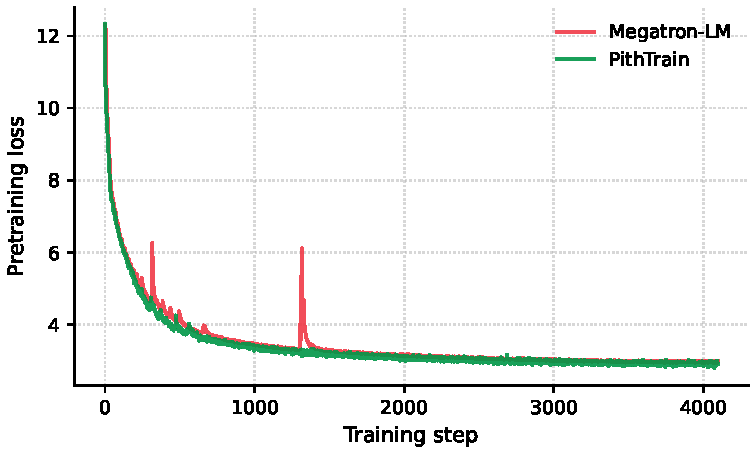
\includegraphics[width=\linewidth]{figures/loss_curve.pdf}
  \end{minipage}
  \caption{Training configuration (left) and pretraining loss curves
  (right) for Qwen3-30B-A3B trained with \megatron and \sys.}
  \label{fig:appendix-loss-curve}
\end{figure}

\subsection{Downstream Accuracy}
\label{sec:appendix:downstream}

We evaluate downstream task accuracy across six standard
benchmarks:
OpenBookQA~\cite{mihaylov2018openbookqa} and
WinoGrande~\cite{sakaguchi2020winogrande} in the 0-shot setting, and
ARC-Challenge, ARC-Easy~\cite{clark2018arc},
HellaSwag~\cite{zellers2019hellaswag}, and PIQA~\cite{bisk2020piqa} in
the 10-shot setting. \autoref{fig:appendix-downstream} plots
accuracy for each task; \megatron and \sys achieve comparable
accuracy within statistical noise across all six benchmarks at every
checkpoint.

\begin{figure}[t]
  \centering
  \begin{subfigure}{0.32\linewidth}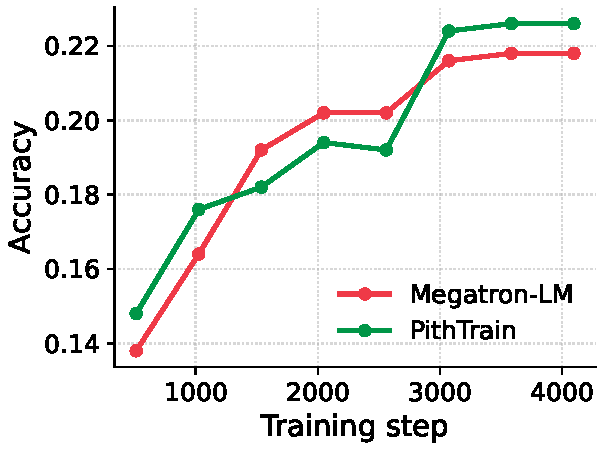
\includegraphics[width=\linewidth]{figures/downstream_openbookqa.pdf}\caption{OpenBookQA (0-shot)}\end{subfigure}
  \hfill
  \begin{subfigure}{0.32\linewidth}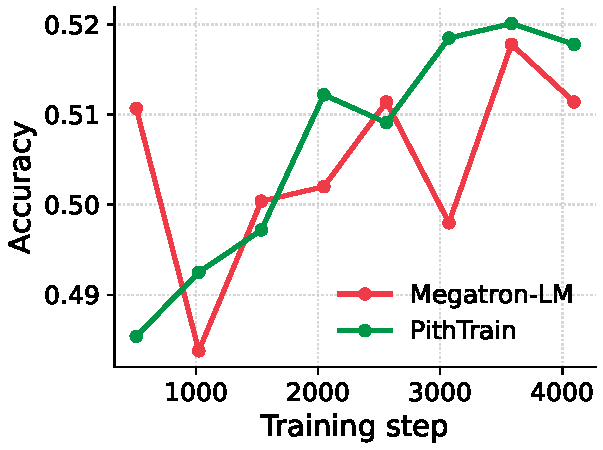
\includegraphics[width=\linewidth]{figures/downstream_winogrande.pdf}\caption{WinoGrande (0-shot)}\end{subfigure}
  \hfill
  \begin{subfigure}{0.32\linewidth}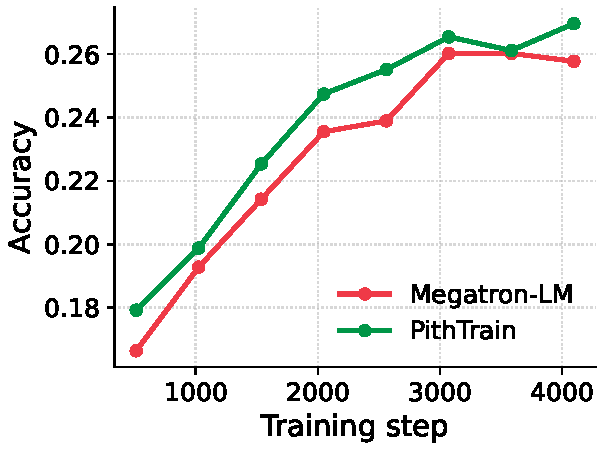
\includegraphics[width=\linewidth]{figures/downstream_arc_challenge.pdf}\caption{ARC-Challenge (10-shot)}\end{subfigure}

  \medskip
  \begin{subfigure}{0.32\linewidth}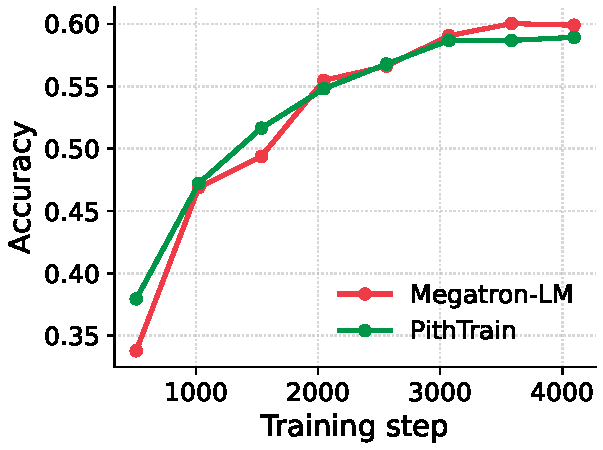
\includegraphics[width=\linewidth]{figures/downstream_arc_easy.pdf}\caption{ARC-Easy (10-shot)}\end{subfigure}
  \hfill
  \begin{subfigure}{0.32\linewidth}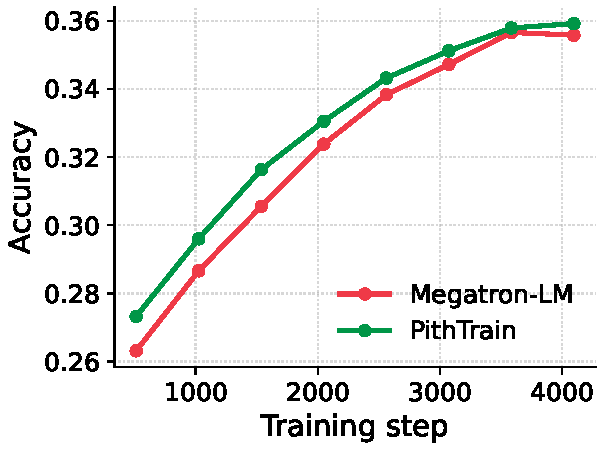
\includegraphics[width=\linewidth]{figures/downstream_hellaswag.pdf}\caption{HellaSwag (10-shot)}\end{subfigure}
  \hfill
  \begin{subfigure}{0.32\linewidth}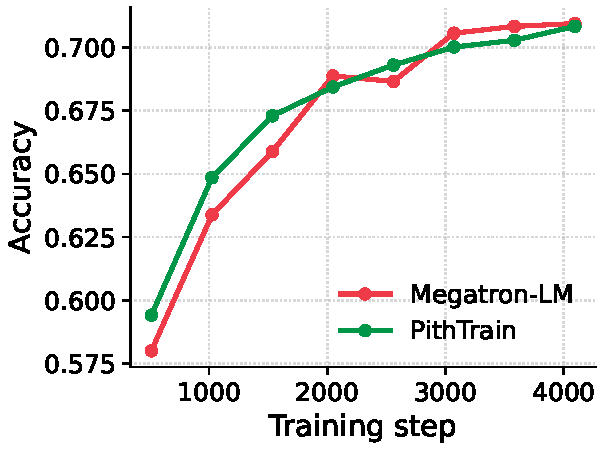
\includegraphics[width=\linewidth]{figures/downstream_piqa.pdf}\caption{PIQA (10-shot)}\end{subfigure}

  \caption{Downstream task accuracy for Qwen3-30B-A3B trained with
  \megatron and \sys.}
  \label{fig:appendix-downstream}
\end{figure}


\section{Task Suite}
\label{sec:appendix:tasks}

This appendix expands the per-category task descriptions and the
correctness checks used to validate each attempt. All
operate-and-profile and new-feature tasks share a fixed training
configuration: the base model is
DeepSeek-V2-Lite~\cite{deepseekai2024deepseekv2strongeconomicalefficient}
(its training fits within a single node with 8 NVIDIA H100 GPUs), the
parallelism mesh is PP=4, EP=2, DP=1, sequence length 2048, global
batch size 1024, precision BF16.

\subsection{Q\&A Tasks}
\label{sec:appendix-codebaseqa}

Each Q\&A task asks the agent to locate where a specific behavior
lives in the framework codebase. The agent receives a single
prompt consisting of the \emph{universal instruction} below followed
verbatim by the full query text for that task (Q1--Q12 in
\S\ref{sec:appendix:tasks:qa-descriptions}), and has read-only access
to \texttt{Read}, \texttt{Grep}, \texttt{Glob}, and \texttt{Bash};
tools that modify the working tree (\texttt{Edit}, \texttt{Write},
\texttt{NotebookEdit}) are explicitly disabled. Correctness is
validated by two independent human graders
(\S\ref{sec:appendix:tasks:qa-correctness}).

\MyPara{Universal instruction (prepended to every query).}
Your task is to explore this training framework codebase and answer
the question that follows. Every claim must be verified against the
code on disk before you state it: use your CLI tools (Read, Grep,
Glob, Bash) to locate the exact symbol, file, and line, then cite the
\texttt{path/to/file.py:LINE} you actually read. Wrap your final
response in \texttt{<final\_answer>} tags, trace the execution path
step by step, and give one citation per claim. If a feature is
genuinely absent from this codebase, say so explicitly and cite
negative evidence (the grep command and pattern that returned zero
matches, or the file you inspected that does not contain it). A
correct ``absent, verified'' answer is preferred over a fabricated
one.

\subsubsection{Task Descriptions}
\label{sec:appendix:tasks:qa-descriptions}

\MyPara{Q1: Process Groups / Device Mesh.}
Trace the sequence of function calls from the main training entry
script down to the initialization of the PyTorch distributed process
groups or DeviceMesh. Detail the exact file paths, function names,
and line numbers where the world size and ranks for the parallel
groups present in this codebase (any of DP, TP, PP, EP, CP that this
repo actually supports) are assigned.

\MyPara{Q2: Configuration Propagation.}
Locate the exact file and line numbers where the user-provided
configuration for \texttt{hidden\_size} or \texttt{dim} is parsed.
Trace how this specific variable propagates down to the instantiation
of the first Transformer block.

\MyPara{Q3: Data Loading \& Sharding.}
Trace the initialization of the dataset and dataloader. Identify the
file, class, and line number where the global dataset is sliced or
partitioned among the Data Parallel ranks to ensure each rank
receives a unique, non-overlapping subset of data.

\MyPara{Q4: Distributed Seed Management.}
Find where the random seeds are set for data loading versus model
initialization. Provide the exact file paths and line numbers, and
trace how seeds are differentiated across different parallel groups
(or, if they are deliberately shared, where and why).

\MyPara{Q5: Attention Kernel Dispatch.}
Locate the core attention module. Trace the logic that selects
between an optimised kernel (FlashAttention, PyTorch SDPA flash
backend, ring attention, etc.) and any fallback math implementation.
Identify the exact file, class, line number, and configuration
flag/condition controlling this dispatch. If the dispatch is
delegated to the PyTorch \texttt{scaled\_dot\_product\_attention}, say
so and cite the call site.

\MyPara{Q6: RoPE Implementation.}
Find where the Rotary Positional Embedding (RoPE) is implemented.
Locate the function that precomputes the frequency tensor
(sine/cosine cache). Provide the file path, class/function name, and
exact line numbers of the tensor operations where the rotary
transform is applied to the Query and Key tensors.

\MyPara{Q7: SwiGLU / MLP Block.}
Locate the Feed-Forward Network (FFN) implementation. Identify the
file and line number where the SwiGLU activation (or equivalent gated
linear unit) is mathematically applied. Trace how the up-projection
tensor is chunked or split before the activation function.

\MyPara{Q8: Normalization Placement.}
Find the implementation of the main Transformer layer. Provide the
file and exact line numbers where the normalization (RMSNorm or
LayerNorm) is applied before the attention module. Detail where the
\texttt{epsilon} (eps) term is added for numerical stability.

\MyPara{Q9: Context / Sequence Parallelism.}
Find where sequence parallelism (or context parallelism) is handled.
Identify the exact file and line numbers where the sequence dimension
of the input tensor is sharded, gathered, or scattered across ranks
during the forward and backward passes. If the codebase does not
support CP/SP, say so and cite the negative evidence.

\MyPara{Q10: FSDP / DDP Wrapping.}
Locate the exact file and line numbers where the core model is
wrapped with Fully Sharded Data Parallel (FSDP1 or FSDP2) or
Distributed Data Parallel (DDP) wrappers, and identify the
device-mesh axes used for sharding/replication.

\MyPara{Q11: Global Gradient Clipping.}
Trace the logic for global gradient norm clipping. Find the file,
function, and exact line number where the global norm of the
gradients is computed (including any reduction across distributed
ranks) before the optimizer step.

\MyPara{Q12: Distributed Checkpoint Serialization.}
Locate the model checkpoint saving logic. Detail whether the system
uses a rank-0 gather approach or distributed sharded saving (e.g.,
PyTorch DCP). Provide the exact file path and line numbers where the
disk serialization occurs.

\subsubsection{Correctness Checks}
\label{sec:appendix:tasks:qa-correctness}

Each Q\&A answer the agent returns cites the file paths, function
names, and line numbers in the framework codebase that implement
the behavior the question asks about. Two human graders
independently trace these citations: they open each cited code
location and verify that the code there does what the agent claims
in the answer. An attempt is recorded as \emph{satisfied} when both
graders confirm every citation against the code on disk;
disagreements are resolved by a third reader who looks only at the
cited evidence. All 108 attempts (12 questions $\times$ 3
frameworks $\times$ 3 attempts) were judged satisfied by both
graders.

\subsection{Operate-and-profile Tasks}
\label{sec:appendix:tasks:operate}

Each operate-and-profile task asks the agent to drive a real
training-system workflow end-to-end, so success requires the agent
to set up the environment, run the framework as intended, and
produce the expected artifact. The four tasks span the workflows
a researcher typically performs before any code change: getting
the framework running, executing a full train-and-evaluate
pipeline, instrumenting the model to capture behavior, and
profiling the system to surface bottlenecks.

\subsubsection{Task Descriptions}
\label{sec:appendix:tasks:operate-descriptions}

\MyPara{Getting Started.}
Set up the Python environment for the framework and run the
provided 5-step smoke training script. Success means the script
reaches step 5 with a finite loss. The agent must install all
dependencies the script needs so that running \texttt{bash
train.sh} as-is succeeds; \texttt{train.sh} itself documents best
practices for training MoE models and is read-only. Pre-tokenized
DCLM and the converted base-model checkpoint are pre-staged.

\MyPara{Train and Evaluate.}
Drive the full setup-train-export-evaluate pipeline for
the base model. The agent trains from random initialization for
25 steps, exports the resulting checkpoint to HuggingFace format,
and runs lm-evaluation-harness HellaSwag (zero-shot) on it via
vLLM. The task tests pipeline correctness, not model quality: the
HellaSwag score is expected to be near-random because 25 steps from
random init produces a barely-trained model, and the agent must
produce \emph{some} score from a working pipeline. Initialization
must be random; everything outside the fixed mesh and step count
(LR, optimizer, scheduler, data preprocessing) is left to the
agent.

\MyPara{Collect Routing Trace.}
Instrument training to dump the per-token MoE routing trace for
the first 8M training tokens. The routing
decision in each MoE layer,
the top-$k$ expert IDs and their gating weights, must be captured
for every token in the global batch. Training resumes from the
released HuggingFace checkpoint so the router is in its trained,
load-balanced regime; routing decisions are model-intrinsic and
valid from step 1, so no warmup is required. The output schema is
one \texttt{step-<step\_id:08d>.npz} file per step under
\texttt{workspace/<framework>/routing-traces/}, each containing the
expert-ID and gating-weight arrays.

\MyPara{Report Heavy Kernels.}
Profile a 7-step training run with Nsight Systems
and identify the top 3 most expensive CUDA kernels by total GPU
time, aggregated across all 8 ranks. Training resumes from the
released HuggingFace checkpoint; the agent profiles only step 7
because steps 1--6 are warmup for cudagraph capture, NCCL
handshake, and allocator priming. The output is a single CSV at
\texttt{workspace/<framework>/heavy-kernels/top-kernels.csv} with
header \texttt{kernel\_name,total\_time\_ms,instances,mean\_time\_ms}
and exactly three rows sorted by \texttt{total\_time\_ms}
descending, plus the raw \texttt{profile.nsys-rep} so the result is
reproducible.

\subsubsection{Correctness Checks}
\label{sec:appendix:tasks:operate-correctness}

Each operate-and-profile task verifies the artifact the agent
produces, not the path the agent took to produce it. We use a
mix of programmatic checks baked into the task harness and human
inspection where the artifact is non-textual.

\MyPara{Getting Started.}
The task succeeds when running \texttt{train.sh} reaches step 5
with a finite loss. After the agent finishes installing
dependencies, the harness re-runs the (read-only) training script
and parses the resulting log; the artifact is accepted only if
step 5 prints a finite loss value.

\MyPara{Train and Evaluate.}
The harness ships a read-only \texttt{evaluate.sh} script that
consumes the pipeline output produced by the agent: the agent
trains for 25
steps from random init, exports the resulting checkpoint to
HuggingFace format, and \texttt{evaluate.sh} loads the export into
vLLM and runs lm-evaluation-harness HellaSwag (zero-shot). An
attempt is satisfied when \texttt{evaluate.sh} runs to completion
and writes a finite HellaSwag score; the score is not required to
clear any quality threshold, since 25 steps from random
initialization is expected to yield near-random accuracy.

\MyPara{Collect Routing Trace.}
The harness verifies that four
\texttt{step-<step\_id:08d>.npz} files are present at
\texttt{workspace/<framework>/routing-traces/} and that each
carries expert-ID and gating-weight arrays of the correct shape
for every MoE layer over every token in the global batch. A
programmatic check additionally confirms that the expert-ID
values are within the valid range \texttt{[0, num\_experts)} for
the MoE configuration of the model, and that the gating weights
are non-negative and sum to 1 over the top-$k$ selected experts
for every token.

\MyPara{Report Heavy Kernels.}
The agent submits both \texttt{top-kernels.csv} and the raw
\texttt{profile.nsys-rep}. The harness checks the CSV
programmatically against the prescribed schema (header, exactly
three rows sorted by total time descending). The kernel names
themselves are validated by a human reader who opens
\texttt{profile.nsys-rep} in the Nsight Systems profiler GUI,
reads the CUDA GPU Kernel Summary in the Stats System view, and
confirms that the top three kernel names in the CSV produced by
the agent match the top three entries shown by the profiler.

All 36 attempts (4 tasks $\times$ 3 frameworks $\times$ 3
attempts) produced an artifact accepted by both the harness and
the human reader.

\subsection{New-feature Tasks}
\label{sec:appendix:tasks:new-feature}

Each new-feature task mimics the workflow of a researcher or ML
engineer integrating a recently published modeling architecture
into a training framework. The agent is given the same materials
such an engineer would normally consult: the arXiv paper and the
reference implementation. From these inputs, the agent must
produce a training script that integrates the new feature into the
base model and runs on DCLM~\cite{li2024dclm} under the fixed
configuration above.

The four tasks are chosen for both coverage and a fair
starting point. Two revise the attention mechanism and two require
changes at the FFN (MoE) layer, so the suite spans the architectural
subsystems a training framework must accommodate. None of the four
architectures had been integrated into any of the three frameworks
we compare at the time of this study, so all frameworks start the
task from the same point and the comparison reflects only how the
design of each framework affects integration effort.

Correctness is validated on two axes. First, the cross-entropy loss
must decrease across the 64-step run and remain finite (no explosion,
no NaN), evidence that the modified training pipeline produces a
learnable model. Second, the changes made by the
agent must satisfy three task-specific rules, each validating one
required component of the new feature
(\S\ref{sec:appendix:tasks:rules}); the rules target the
architectural elements that distinguish each new feature from the
baseline framework, ensuring the agent has implemented the intended
mechanism rather than producing a passing-loss reading from an
unchanged model. An attempt is recorded as \emph{satisfied} when both
axes hold.

\subsubsection{Task Descriptions}
\label{sec:appendix:tasks:descriptions}

\MyPara{Diff~\cite{ye2024differential}.}
Differential attention replaces a single softmax-attention map with
the difference of two parallel softmax maps,
$\mathrm{Attn}(Q,K,V) = (\mathrm{softmax}(Q_1 K_1^\top) - \lambda\,
\mathrm{softmax}(Q_2 K_2^\top))\,V$, where $\lambda$ is a learned
per-head scalar. The construction cancels common-mode attention
noise, sharpening which tokens receive mass. Integrating it
involves splitting the per-head $Q$/$K$ projections in half and
introducing $\lambda$ as a trainable parameter with the published
initialisation schedule.

\MyPara{DynMoE~\cite{guo2024dynamic}.}
Standard MoE fixes the number of activated experts $k$ per token.
DynMoE replaces top-$k$ selection with a per-expert sigmoid gate and
a learned threshold, so the count of active experts varies per
token. Integrating it involves replacing the top-$k$ routing
kernel of the framework and reformulating the load-balancing
auxiliary loss for a variable-$k$ regime.

\MyPara{MoBA~\cite{lu2025moba}.}
MoBA partitions the key/value sequence into fixed-size blocks
and routes each query to the top-$k$ blocks
selected by a learned gate, yielding sub-quadratic attention
cost in the sequence length. Integrating it involves
inserting block-level routing between the $Q$/$K$ projection and
the attention computation, composing with the existing attention
backend in the framework, and preserving
causal masking inside each selected block.

\MyPara{MoE++~\cite{jin2025moeplusplus}.}
MoE++ augments a standard MoE expert pool with three
zero-computation expert types (\emph{zero}, \emph{copy}, and
\emph{constant}), allowing easy tokens to be routed past the
feed-forward layer entirely. Integrating it involves extending the
expert pool definition with the zero-computation variants, widening
the router output to cover them, and adjusting the load-balancing
loss to prevent the zero experts from absorbing all easy tokens.

\subsubsection{Rule-based Correctness Checks}
\label{sec:appendix:tasks:rules}

Each new-feature task decomposes into three required components,
the architectural elements that distinguish the new feature from
the baseline framework. The rules below name each component and
describe how it should be implemented; they were fixed before
inspecting any attempt. Each
attempt is judged by an independent
\texttt{claude-opus-4-7} session at \texttt{xhigh} effort, given
the three rules and the git diff produced by the agent against the
main branch of the framework; the judge returns PASS or FAIL per
rule with a one-sentence justification quoting a specific code
reference, and an attempt is recorded as \emph{satisfied} when all
three rules pass. We additionally inspect every verdict and its
cited justification by hand: a human reader opens the diff at the
cited file and confirms the line evidence for both PASS judgements
and any FAIL or partial verdicts. Across all 36 attempts
(4 tasks $\times$ 3 frameworks $\times$ 3 attempts), every attempt
satisfies all three rules of its task.

\MyPara{Diff.}
\begin{itemize}
  \setlength\itemsep{1pt}
  \item[R1.] The attention forward path produces two separate softmax outputs that are combined as $\mathrm{attn}_1 - \lambda \cdot \mathrm{attn}_2$ (literal subtraction with a learnable coefficient).
  \item[R2.] A learnable parameter ($\lambda$, e.g.\ named \texttt{lambda} or \texttt{lambda\_init}) is registered as an \texttt{nn.Parameter} with shape compatible with per-head broadcasting.
  \item[R3.] The $Q$/$K$ projections are split into two halves, either via an output dimension of $2 \cdot n_\mathrm{heads} \cdot d_\mathrm{head}$ followed by a split, or via two separate projection layers.
\end{itemize}

\MyPara{DynMoE.}
\begin{itemize}
  \setlength\itemsep{1pt}
  \item[R1.] The router uses per-expert sigmoid gates (or sigmoid-gated activation), not pure softmax with top-$k$ selection.
  \item[R2.] A learnable threshold parameter for expert activation is registered as an \texttt{nn.Parameter} (often named \texttt{tau}, \texttt{threshold}, or \texttt{gate\_threshold}).
  \item[R3.] Active-expert selection is not a fixed \texttt{top\_k = N}; the count depends on which experts pass the threshold (boolean mask or variable-length selection).
\end{itemize}

\MyPara{MoBA.}
\begin{itemize}
  \setlength\itemsep{1pt}
  \item[R1.] The $K$/$V$ sequence is partitioned into fixed-size blocks (a \texttt{reshape} or \texttt{view} into shape \texttt{[\dots, $n_\mathrm{blocks}$, $B$, \dots]} or equivalent).
  \item[R2.] Each query computes a per-block score (typically $\mathrm{query} \cdot \mathrm{pooled\_block\_key}$) followed by top-$k$ block selection.
  \item[R3.] Final attention is computed only over the selected blocks, with causal masking preserved at block boundaries (each query attends only to blocks at positions $\leq$ its own).
\end{itemize}

\MyPara{MoE++.}
\begin{itemize}
  \setlength\itemsep{1pt}
  \item[R1.] The expert pool includes at least one zero-computation expert type (\emph{zero}, \emph{copy}, or \emph{constant}), identifiable by class name, string literal, or a specialised expert factory.
  \item[R2.] The router emits logits over a pool that contains both regular FFN experts and zero-computation experts, so the router learns to dispatch tokens to the no-op variants. The zero-computation experts may be added on top of the existing pool (router output dim grows to $n_{\mathrm{FFN}} + n_{\mathrm{zero}}$) or carved out of an unchanged total expert count.
  \item[R3.] The load-balancing auxiliary loss handles zero experts explicitly: they are excluded from the balance term, weighted differently, or balanced under a separate penalty.
\end{itemize}

\section{Per-Task Results}
\label{sec:appendix:per-task-results}

This appendix reports per-attempt agent effort across the three
task categories: Tables~\ref{tab:appendix-per-attempt-codebaseqa}
and~\ref{tab:appendix-per-attempt-codebaseqa-2} cover the 12 Q\&A
tasks (split 6/6 across two pages),
\autoref{tab:appendix-per-attempt-operate} covers the four
operate-and-profile tasks, and
\autoref{tab:appendix-per-attempt-new-feature} covers the four
new-feature tasks. Each row is one independent attempt;
per-task medians appear in the corresponding main-text tables in
\S\ref{sec:eval:agent}. Session Duration and Active GPU Time are
reported in minutes. Lower is better on every metric.

\begin{table}[t]
  \centering
  \footnotesize
  \caption{Per-attempt agent effort on the Q\&A tasks Q1--Q6 (\S\ref{sec:eval:agent}). Each row is one independent attempt. Session Duration is in minutes.}
  \label{tab:appendix-per-attempt-codebaseqa}
  \setlength{\tabcolsep}{4pt}
  \begin{tabular}{@{}llr|rrrr@{}}
    \toprule
    Task
      & Framework
      & Attempt
      & \makecell[br]{Session\\Duration}
      & \makecell[br]{Agent\\Turns}
      & \makecell[br]{Per-Turn\\Context}
      & \makecell[br]{Output\\Tokens} \\
    \midrule
    \multirow{9}{*}{Q1: Process Groups / Device Mesh}
      & \megatron     & 1st & 2.0 & 33 & 47.8K & 9.0K \\
      &                               & 2nd & 2.2 & 26 & 45.8K & 9.7K \\
      &                               & 3rd & 2.1 & 34 & 44.5K & 9.0K \\
      & \torchtitan   & 1st & 2.8 & 18 & 44.3K & 7.1K \\
      &                               & 2nd & 3.1 & 19 & 45.2K & 7.0K \\
      &                               & 3rd & 3.0 & 15 & 42.9K & 7.3K \\
      & \sys          & 1st & 1.6 & 15 & 33.4K & 4.1K \\
      &                               & 2nd & 1.4 & 13 & 33.1K & 3.5K \\
      &                               & 3rd & 2.0 & 17 & 35.1K & 5.3K \\
    \midrule
    \multirow{9}{*}{Q2: Configuration Propagation}
      & \megatron     & 1st & 2.9 & 54 & 43.4K & 10.7K \\
      &                               & 2nd & 1.9 & 37 & 37.6K & 8.4K \\
      &                               & 3rd & 3.2 & 54 & 41.2K & 12.0K \\
      & \torchtitan   & 1st & 2.8 & 25 & 42.6K & 6.4K \\
      &                               & 2nd & 3.0 & 34 & 43.5K & 7.8K \\
      &                               & 3rd & 3.5 & 28 & 45.0K & 9.2K \\
      & \sys          & 1st & 2.0 & 18 & 35.7K & 4.5K \\
      &                               & 2nd & 2.9 & 28 & 35.9K & 7.6K \\
      &                               & 3rd & 2.2 & 18 & 36.8K & 5.4K \\
    \midrule
    \multirow{9}{*}{Q3: Data Loading \& Sharding}
      & \megatron     & 1st & 1.0 & 10 & 32.1K & 3.8K \\
      &                               & 2nd & 0.8 & 14 & 31.3K & 3.0K \\
      &                               & 3rd & 0.9 & 14 & 30.8K & 3.4K \\
      & \torchtitan   & 1st & 1.2 & 14 & 35.0K & 3.2K \\
      &                               & 2nd & 1.8 & 21 & 38.2K & 4.0K \\
      &                               & 3rd & 1.2 & 14 & 36.1K & 3.5K \\
      & \sys          & 1st & 1.4 & 13 & 34.5K & 3.5K \\
      &                               & 2nd & 1.3 & 15 & 29.1K & 3.4K \\
      &                               & 3rd & 1.5 & 8 & 34.1K & 2.9K \\
    \midrule
    \multirow{9}{*}{Q4: Distributed Seed Management}
      & \megatron     & 1st & 2.2 & 36 & 37.5K & 8.8K \\
      &                               & 2nd & 2.2 & 37 & 49.4K & 10.0K \\
      &                               & 3rd & 2.5 & 34 & 41.3K & 10.4K \\
      & \torchtitan   & 1st & 3.1 & 22 & 37.9K & 6.5K \\
      &                               & 2nd & 3.3 & 26 & 39.7K & 6.9K \\
      &                               & 3rd & 3.9 & 32 & 41.7K & 7.9K \\
      & \sys          & 1st & 2.2 & 15 & 34.0K & 5.0K \\
      &                               & 2nd & 2.3 & 19 & 31.1K & 5.2K \\
      &                               & 3rd & 2.5 & 16 & 30.7K & 5.6K \\
    \midrule
    \multirow{9}{*}{Q5: Attention Kernel Dispatch}
      & \megatron     & 1st & 3.7 & 63 & 56.0K & 14.0K \\
      &                               & 2nd & 2.8 & 48 & 46.5K & 10.7K \\
      &                               & 3rd & 1.7 & 27 & 39.8K & 6.6K \\
      & \torchtitan   & 1st & 2.1 & 20 & 41.7K & 4.8K \\
      &                               & 2nd & 2.0 & 19 & 43.7K & 5.1K \\
      &                               & 3rd & 2.0 & 15 & 41.2K & 4.7K \\
      & \sys          & 1st & 1.9 & 20 & 34.2K & 4.4K \\
      &                               & 2nd & 1.9 & 24 & 33.7K & 4.6K \\
      &                               & 3rd & 2.0 & 21 & 33.8K & 5.0K \\
    \midrule
    \multirow{9}{*}{Q6: RoPE Implementation}
      & \megatron     & 1st & 1.1 & 12 & 36.4K & 4.5K \\
      &                               & 2nd & 1.1 & 12 & 35.9K & 4.5K \\
      &                               & 3rd & 0.9 & 12 & 36.4K & 3.2K \\
      & \torchtitan   & 1st & 0.7 & 4 & 29.9K & 1.9K \\
      &                               & 2nd & 1.0 & 4 & 29.9K & 2.6K \\
      &                               & 3rd & 1.0 & 4 & 29.9K & 2.3K \\
      & \sys          & 1st & 1.2 & 8 & 26.7K & 2.6K \\
      &                               & 2nd & 1.3 & 11 & 27.9K & 3.3K \\
      &                               & 3rd & 2.0 & 18 & 31.8K & 5.6K \\
    \bottomrule
  \end{tabular}
\end{table}

\begin{table}[t]
  \centering
  \footnotesize
  \caption{Per-attempt agent effort on the Q\&A tasks (continued, Q7--Q12).}
  \label{tab:appendix-per-attempt-codebaseqa-2}
  \setlength{\tabcolsep}{4pt}
  \begin{tabular}{@{}llr|rrrr@{}}
    \toprule
    Task
      & Framework
      & Attempt
      & \makecell[br]{Session\\Duration}
      & \makecell[br]{Agent\\Turns}
      & \makecell[br]{Per-Turn\\Context}
      & \makecell[br]{Output\\Tokens} \\
    \midrule
    \multirow{9}{*}{Q7: SwiGLU / MLP Block}
      & \megatron     & 1st & 1.0 & 10 & 31.5K & 3.2K \\
      &                               & 2nd & 0.7 & 8 & 31.4K & 2.5K \\
      &                               & 3rd & 0.7 & 9 & 34.1K & 2.6K \\
      & \torchtitan   & 1st & 1.6 & 11 & 30.0K & 3.2K \\
      &                               & 2nd & 1.4 & 13 & 30.2K & 3.8K \\
      &                               & 3rd & 0.9 & 12 & 30.0K & 3.4K \\
      & \sys          & 1st & 2.1 & 15 & 31.5K & 4.6K \\
      &                               & 2nd & 1.6 & 13 & 40.3K & 4.2K \\
      &                               & 3rd & 1.5 & 14 & 30.1K & 3.8K \\
    \midrule
    \multirow{9}{*}{Q8: Normalization Placement}
      & \megatron     & 1st & 1.0 & 15 & 30.3K & 4.1K \\
      &                               & 2nd & 2.6 & 20 & 30.8K & 4.7K \\
      &                               & 3rd & 1.5 & 25 & 34.2K & 5.5K \\
      & \torchtitan   & 1st & 1.0 & 11 & 32.7K & 3.5K \\
      &                               & 2nd & 0.7 & 8 & 30.3K & 2.5K \\
      &                               & 3rd & 1.1 & 14 & 33.7K & 3.5K \\
      & \sys          & 1st & 1.1 & 9 & 27.7K & 3.0K \\
      &                               & 2nd & 1.3 & 9 & 28.7K & 3.2K \\
      &                               & 3rd & 1.4 & 11 & 29.9K & 3.6K \\
    \midrule
    \multirow{9}{*}{Q9: Context / Sequence Parallelism}
      & \megatron     & 1st & 4.7 & 60 & 45.6K & 6.8K \\
      &                               & 2nd & 3.1 & 34 & 45.2K & 7.6K \\
      &                               & 3rd & 3.3 & 29 & 44.6K & 7.8K \\
      & \torchtitan   & 1st & 1.5 & 20 & 38.6K & 5.8K \\
      &                               & 2nd & 2.0 & 16 & 38.6K & 7.5K \\
      &                               & 3rd & 1.6 & 16 & 37.1K & 6.0K \\
      & \sys          & 1st & 2.9 & 22 & 37.6K & 7.1K \\
      &                               & 2nd & 2.2 & 16 & 37.0K & 5.1K \\
      &                               & 3rd & 1.7 & 16 & 35.1K & 4.1K \\
    \midrule
    \multirow{9}{*}{Q10: FSDP / DDP Wrapping}
      & \megatron     & 1st & 2.8 & 19 & 37.8K & 7.0K \\
      &                               & 2nd & 2.3 & 21 & 38.6K & 5.6K \\
      &                               & 3rd & 2.7 & 16 & 35.5K & 5.9K \\
      & \torchtitan   & 1st & 1.6 & 24 & 44.1K & 6.0K \\
      &                               & 2nd & 1.3 & 17 & 36.7K & 4.9K \\
      &                               & 3rd & 1.5 & 16 & 38.8K & 5.1K \\
      & \sys          & 1st & 1.1 & 9 & 26.9K & 2.6K \\
      &                               & 2nd & 1.2 & 12 & 30.2K & 2.9K \\
      &                               & 3rd & 1.4 & 11 & 29.4K & 3.0K \\
    \midrule
    \multirow{9}{*}{Q11: Global Gradient Clipping}
      & \megatron     & 1st & 1.4 & 10 & 31.9K & 3.2K \\
      &                               & 2nd & 1.2 & 12 & 31.3K & 3.1K \\
      &                               & 3rd & 1.0 & 10 & 31.0K & 2.9K \\
      & \torchtitan   & 1st & 0.7 & 9 & 30.0K & 2.5K \\
      &                               & 2nd & 0.7 & 8 & 30.2K & 2.7K \\
      &                               & 3rd & 0.7 & 7 & 30.1K & 2.5K \\
      & \sys          & 1st & 0.8 & 6 & 25.6K & 2.0K \\
      &                               & 2nd & 0.8 & 7 & 25.8K & 1.9K \\
      &                               & 3rd & 0.8 & 6 & 25.5K & 2.0K \\
    \midrule
    \multirow{9}{*}{Q12: Distributed Checkpoint Serialization}
      & \megatron     & 1st & 2.0 & 19 & 37.2K & 5.1K \\
      &                               & 2nd & 1.8 & 18 & 36.2K & 4.5K \\
      &                               & 3rd & 2.8 & 17 & 37.1K & 6.4K \\
      & \torchtitan   & 1st & 0.6 & 5 & 33.9K & 2.2K \\
      &                               & 2nd & 0.8 & 5 & 33.9K & 2.6K \\
      &                               & 3rd & 0.6 & 5 & 33.9K & 2.2K \\
      & \sys          & 1st & 1.2 & 10 & 31.1K & 2.5K \\
      &                               & 2nd & 1.1 & 9 & 30.0K & 2.6K \\
      &                               & 3rd & 1.4 & 10 & 35.3K & 2.8K \\
    \bottomrule
  \end{tabular}
\end{table}

\begin{table}[t]
  \centering
  \footnotesize
  \caption{Per-attempt agent effort on the operate-and-profile tasks (\S\ref{sec:eval:agent}). Each row is one independent attempt. Session Duration and Active GPU Time are in minutes.}
  \label{tab:appendix-per-attempt-operate}
  \setlength{\tabcolsep}{4pt}
  \begin{tabular}{@{}llr|rrrrr@{}}
    \toprule
    Task
      & Framework
      & Attempt
      & \makecell[br]{Session\\Duration}
      & \makecell[br]{Active\\GPU Time}
      & \makecell[br]{Agent\\Turns}
      & \makecell[br]{Per-Turn\\Context}
      & \makecell[br]{Output\\Tokens} \\
    \midrule
    \multirow{9}{*}{Getting Started}
      & \megatron    & 1st & 47.6 & 5.9 & 106 & 85.5K & 31.9K \\
      &                               & 2nd & 40.5 & 5.4 & 88 & 69.5K & 26.9K \\
      &                               & 3rd & 24.1 & 5.2 & 78 & 64.0K & 25.8K \\
      & \torchtitan  & 1st & 10.8 & 5.0 & 54 & 62.0K & 15.8K \\
      &                               & 2nd & 11.4 & 5.2 & 47 & 43.1K & 15.4K \\
      &                               & 3rd & 13.5 & 5.6 & 68 & 56.8K & 18.3K \\
      & \sys         & 1st & 7.6 & 3.9 & 20 & 33.8K & 5.4K \\
      &                               & 2nd & 6.6 & 3.0 & 26 & 37.0K & 5.8K \\
      &                               & 3rd & 5.8 & 3.1 & 28 & 37.9K & 7.6K \\
    \midrule
    \multirow{9}{*}{Train and Evaluate}
      & \megatron    & 1st & 52.3 & 29.3 & 163 & 109.2K & 45.1K \\
      &                               & 2nd & 58.8 & 36.0 & 155 & 101.4K & 53.2K \\
      &                               & 3rd & 55.5 & 38.1 & 170 & 106.4K & 52.9K \\
      & \torchtitan  & 1st & 59.5 & 36.3 & 212 & 176.6K & 75.8K \\
      &                               & 2nd & 101.6 & 87.5 & 268 & 149.8K & 97.8K \\
      &                               & 3rd & 72.5 & 28.8 & 198 & 197.1K & 109.3K \\
      & \sys         & 1st & 42.0 & 25.9 & 100 & 86.5K & 36.9K \\
      &                               & 2nd & 37.1 & 22.7 & 87 & 83.1K & 34.2K \\
      &                               & 3rd & 38.5 & 19.3 & 92 & 85.5K & 32.3K \\
    \midrule
    \multirow{9}{*}{Collect Routing Trace}
      & \megatron    & 1st & 33.3 & 8.3 & 112 & 144.3K & 102.1K \\
      &                               & 2nd & 33.3 & 5.5 & 138 & 158.8K & 102.5K \\
      &                               & 3rd & 25.1 & 5.3 & 87 & 106.4K & 74.7K \\
      & \torchtitan  & 1st & 32.8 & 10.4 & 93 & 166.0K & 84.7K \\
      &                               & 2nd & 41.4 & 11.9 & 152 & 181.7K & 113.6K \\
      &                               & 3rd & 30.8 & 9.8 & 103 & 160.3K & 74.8K \\
      & \sys         & 1st & 16.3 & 2.7 & 58 & 118.7K & 56.2K \\
      &                               & 2nd & 14.3 & 2.8 & 52 & 107.8K & 48.4K \\
      &                               & 3rd & 20.1 & 2.8 & 70 & 146.8K & 71.9K \\
    \midrule
    \multirow{9}{*}{Report Heavy Kernels}
      & \megatron    & 1st & 23.4 & 12.5 & 62 & 67.0K & 31.0K \\
      &                               & 2nd & 22.1 & 12.1 & 53 & 48.1K & 20.5K \\
      &                               & 3rd & 21.2 & 12.0 & 60 & 52.6K & 23.9K \\
      & \torchtitan  & 1st & 14.8 & 8.1 & 44 & 65.1K & 17.0K \\
      &                               & 2nd & 15.0 & 4.8 & 40 & 69.0K & 22.5K \\
      &                               & 3rd & 15.2 & 6.7 & 39 & 66.1K & 22.7K \\
      & \sys         & 1st & 11.8 & 3.7 & 42 & 50.2K & 19.0K \\
      &                               & 2nd & 10.4 & 3.6 & 36 & 44.0K & 11.6K \\
      &                               & 3rd & 12.5 & 3.5 & 43 & 49.2K & 16.0K \\
    \bottomrule
  \end{tabular}
\end{table}

\begin{table}[t]
  \centering
  \footnotesize
  \caption{Per-attempt agent effort on the new-feature tasks (\S\ref{sec:eval:agent}). Each row is one independent attempt. Session Duration and Active GPU Time are in minutes.}
  \label{tab:appendix-per-attempt-new-feature}
  \setlength{\tabcolsep}{4pt}
  \begin{tabular}{@{}llr|rrrrr@{}}
    \toprule
    Task
      & Framework
      & Attempt
      & \makecell[br]{Session\\Duration}
      & \makecell[br]{Active\\GPU Time}
      & \makecell[br]{Agent\\Turns}
      & \makecell[br]{Per-Turn\\Context}
      & \makecell[br]{Output\\Tokens} \\
    \midrule
    \multirow{9}{*}{Diff~\cite{ye2024differential}}
      & \megatron    & 1st & 47.1 & 33.7 & 62 & 118.7K & 49.4K \\
      &                               & 2nd & 56.6 & 44.9 & 125 & 165.9K & 58.3K \\
      &                               & 3rd & 46.3 & 33.6 & 141 & 103.6K & 57.1K \\
      & \torchtitan  & 1st & 49.6 & 40.3 & 61 & 96.9K & 35.4K \\
      &                               & 2nd & 57.1 & 49.2 & 53 & 105.9K & 36.0K \\
      &                               & 3rd & 48.6 & 40.1 & 58 & 103.2K & 38.7K \\
      & \sys         & 1st & 35.3 & 27.6 & 47 & 53.9K & 29.4K \\
      &                               & 2nd & 38.2 & 33.2 & 35 & 69.5K & 22.1K \\
      &                               & 3rd & 42.8 & 27.3 & 83 & 93.0K & 25.4K \\
    \midrule
    \multirow{9}{*}{DynMoE~\cite{guo2024dynamic}}
      & \megatron    & 1st & 84.2 & 45.4 & 200 & 177.9K & 125.3K \\
      &                               & 2nd & 76.7 & 49.1 & 199 & 238.1K & 115.2K \\
      &                               & 3rd & 83.8 & 62.1 & 186 & 208.0K & 94.5K \\
      & \torchtitan  & 1st & 143.6 & 97.8 & 253 & 306.1K & 161.3K \\
      &                               & 2nd & 140.6 & 94.4 & 126 & 211.4K & 178.2K \\
      &                               & 3rd & 115.5 & 90.3 & 197 & 228.8K & 113.5K \\
      & \sys         & 1st & 57.1 & 41.9 & 76 & 146.0K & 52.9K \\
      &                               & 2nd & 61.4 & 42.3 & 73 & 101.4K & 76.4K \\
      &                               & 3rd & 60.4 & 41.3 & 118 & 224.9K & 96.8K \\
    \midrule
    \multirow{9}{*}{MoBA~\cite{lu2025moba}}
      & \megatron    & 1st & 71.1 & 49.1 & 134 & 146.7K & 53.8K \\
      &                               & 2nd & 61.6 & 49.5 & 135 & 108.1K & 56.1K \\
      &                               & 3rd & 59.1 & 49.9 & 91 & 120.9K & 45.7K \\
      & \torchtitan  & 1st & 53.7 & 39.4 & 61 & 110.2K & 54.4K \\
      &                               & 2nd & 138.9 & 107.6 & 104 & 186.2K & 111.8K \\
      &                               & 3rd & 105.1 & 77.9 & 91 & 166.9K & 112.2K \\
      & \sys         & 1st & 38.0 & 27.7 & 57 & 66.4K & 32.4K \\
      &                               & 2nd & 52.9 & 32.0 & 55 & 69.0K & 22.8K \\
      &                               & 3rd & 38.7 & 26.9 & 66 & 81.5K & 50.8K \\
    \midrule
    \multirow{9}{*}{MoE++~\cite{jin2025moeplusplus}}
      & \megatron    & 1st & 144.6 & 78.0 & 829 & 516.5K & 326.4K \\
      &                               & 2nd & 88.5 & 58.7 & 145 & 170.8K & 117.0K \\
      &                               & 3rd & 75.5 & 53.6 & 140 & 188.7K & 86.9K \\
      & \torchtitan  & 1st & 95.2 & 72.1 & 85 & 134.3K & 66.0K \\
      &                               & 2nd & 71.4 & 51.9 & 87 & 164.6K & 85.3K \\
      &                               & 3rd & 63.5 & 45.2 & 125 & 173.4K & 90.4K \\
      & \sys         & 1st & 63.0 & 36.7 & 141 & 176.6K & 107.7K \\
      &                               & 2nd & 63.0 & 39.9 & 85 & 201.0K & 100.2K \\
      &                               & 3rd & 67.7 & 40.1 & 90 & 165.4K & 119.1K \\
    \bottomrule
  \end{tabular}
\end{table}
